\section{Definitions} \label{chapter3:definitions}

The continuous growth and sustainability offered by a platform relies on three criteria.
This section defines these tree criteria, as well as all the underlying concepts.

Additionally, for the context of this thesis, a fourth criterium appear.
It is important for the analyzed platforms to be web compliant.\nt{I don't know where to put this criterium}

\begin{itemize}
\item Maintainability
\item Performance Efficiency
\item Adoption
\item Web compliance
\end{itemize}

\subsection{Maintainability}

\textit{Software maintainability is defined as the degree to which an application is understood, repaired, or enhanced.}\ftnt{http://www.castsoftware.com/glossary/software-maintainability}
% For an application to be maintainable, it needs to be modular.
%Maintainability relies on modularity.
For an application to be maintainable, its frameworks need to enforce modularity directly in the design.
Modularity allows to limit the understanding required to contribute to a module \cite{Stevens1974}.
Which helps developers to repair and enhance the application. 
Moreover, it reduces development time by allowing several developers to simultaneously implement different modules \cite{Wong2009,Cataldo2006}.
% It relies on two factors, module encapsulation and module composition.

\subsubsection{Modularity}

The modularity of a software implementation is about encapsulating subproblems and composing them.
It allows greater design to emerge from the composition of smaller components.

The criteria to define modules to improve maintainability are low coupling and high cohesion \cite{Stevens1974}.
Coupling defines the strength of the interdependence between modules.
Cohesion defines how strongly the features inside a module are related.
% Encapsulating a subproblem into a module helps increase cohesion.
% Composition abstractions helps decrease their coupling.
The composition of modules help decrease coupling, and encapsulation helps increase their cohesion.
Encapsulation and composition improves maintainability.

\begin{itemize}
\item Encapsulation $\to$ High Cohesion
\item Composition $\to$ Low Coupling
\end{itemize}

\subsubsection{Encapsulation}

\paragraph{Boundary Definition}

\illustration{spaghetti programming}
Modular Programming stands upon Structured Programming \cite{Dijkstra1970}.
% Dijkstra firstly developed the concept of Structured Programming \cite{Dijkstra1970}, which later led to modular programming.
% It is defined as \textit{the systematic use of abstraction to control a mass of details, and also a means of documentation which aids program design} \cite{Knuth1974}.
It draws clear interfaces around a piece of implementation so that the execution is enclosed inside.
At a fine level, it helps avoid spaghetti code \cite{Dijkstra1968a}, and at a coarser level, it structures the implementation \cite{Dijkstra1968} into modules, or layers.
% The next paragraph explains further the criteria to draw the borders around modules.

\paragraph{Data Protection}

\illustration{lasagna programming}
Encapsulate a specific design choice in each module, so that it is responsible for one and only one concern, isolate its evolution from impacting the rest of the implementation \cite{Parnas1972, Tarr1999, Hursch1995}.
Examples of such separation of concerns are the separation of the form and the content in HTML / CSS, or the OSI model for the network stack.

\subsubsection{Composition} \label{chapter3:software-maintainability:modularity:features}

\paragraph{Higher-Order Programming}
\nt{If possible, include this reference : Continuations and coroutines \cite{Haynes1984}}

Higher-order programming allows to manipulate functions like any other primary value : to store them in variables, or to pass them as arguments.
It replaces the need for most modern object oriented programming design patterns \ftnt{http://stackoverflow.com/a/5797892/933670} with Inversion of Control \cite{Johnson}, the Hollywood Principle \cite{Sweet1985}, and Monads \cite{Wadler1992}.
Higher-order programming help loosen coupling, thus improve maintainability.

In languages allowing mutable state, higher-order functions are implemented as closure, to preserve the lexical scope \cite{Sussman1998}.
A closure is the association of a function and a reference to the lexical context from its creation.
It allows this function to access variable from this context, even when invoked outside the scope of this context.
\nt{next sentence is redundant with the suit}
It eventually tangles the memory references so that it requires a global memory.

\paragraph{Lazy Evaluation}

Lazy evaluation is an evaluation strategy allowing to defer the execution of a function only when its result is needed.
% And according to \cite{Hughes1989}, \textit{Abelson and Sussman stress that streams (lazy list) is a powerful tool for structuring programs \cite{Sussman1983}.
The lazy evaluation of lists is equivalent to a stream with a null-sized buffer, while the opposite, eager evaluation, corresponds to an infinite buffer \cite{VanRoy2003}.
\nt{find another transition}Indeed, the dataflow programming paradigm resulting from lazy lists is particularly adapted for stream processing applications.

\nt{This paragraph is not very clear}
The lazy evaluation, as well as streams are powerful tools for structuring modular programs \cite{Sussman1983}.
Lazy evaluation allows the execution to be organized as a concurrent pipeline, as the stages are executed independently for each element of the stream.
But this concurrency requires immutability of state, or at least isolation of side-effects.\nt{why ? explain or point to the explanation}
The next section addresses the consequences of higher-order programming and lazy evaluation on parallelism.



\paragraph{}

Finally, the criteria for Maintainability are the following.

\begin{itemize}
\item Encapsulation $\to$ High Cohesion
  \subitem Boundary definition
  \subitem Data protection
\item Composition $\to$ Low Coupling
  \subitem Higher-order programming, Lambda Expressions
  \subitem Lazy evaluation, Stream composition
\end{itemize}


\subsection{Performance Efficiency}

The performance efficiency of a software project is the relation between the usage made of available resources and the delivered performance.
For an application to perform efficiently, the frameworks used need to enforce scalability directly in its design.

Scalability relies on the commutativity of operations execution \cite{Clements2013a}.
Operations are commutative if the order of their executions is irrelevant for the correctness of their results.
Commutativity assures the independence of operations.

\subsubsection{Independence}

The independence, and commutativity of an operations depends on its access to state shared with other operations.
If the operations doesn't rely on any shared state, it is independent.
If it relies on shared state for read or modification, it needs to manage the timing of its execution with the other operations to avoid conflicting accesses.
That is to synchronize with the other operations, which implies communications.

The independence of operations allows to execute them in parallel, hence to deliver performance proportionally to used resources \cite{Amdahl1967,Gunther1993}.
But if the operations are not independent, the communication overhead due to synchronization might occult the performance increase gained by the parallel execution.
If the two operations frequently access the state, then the communications overhead is greater than the performance gain.
On the other hand, if the operations hardly ever access the state, then the communication overhead is compensated by the performance gain.
Because states tend to be shared locally, the operations at a fine-grain level induce a greater communication overhead than the operations at a coarser-level. 
% \subsubsection{Sequentiality or Parallelism}
% In practice, all operations can not be made independent, particularly at a fine-grain level.
% Enforcing parallelism at this fine-grain level induces overhead because of the synchronization between operations.

Therefore, performance efficiency requires the combination of fine-level state sharing to avoid communication overhead, and coarse-level independence to avoid synchronization overhead \cite{Gustafson1988,Gunther1996,Nelson1996,Gunther2002}.
The operations need to be independent at a coarse-grain level, and to be scheduled sequentially at a fine-grain level.

\begin{itemize}
\item Fine-level state sharing\\
  \subitem State mutability
  \subitem $\to$ Sequentiality
\item Coarse-level independence\\
  \subitem State immutability
  \subitem $\to$ Message-passing
\end{itemize}

\subsubsection{Atomicity, Concurrency and Asynchronism}
TODO

\subsubsection{Message-Passing}
TODO


\subsubsection{Modules and Operations}

On the difference between modules encapsulation and operations independence.

Encapsulation aims not to provide this decomposition between sharing and immutable space required for performance scalability.
It aims to draw a clear boundary around the concern of a module to help understanding it.
To allow higher-order programming and mutable state, despite encapsulation, languages implement closures, and intermingle the memory between modules.
It reinforces the need for synchronization and sequentiality.






\subsection{Adoption}

% A software project is maintainable only if there is people willing to maintain it.
An application is sustainable only if the frameworks used to build it generate activity between a community of passionate and the industry.
A framework needs to present a balance between maintainability and performance effiency to be adopted by both the community and the industry.
The maintainability is required for a framework to be appealing to gather a community to support the ecosystem around it.
And the performance efficiency is required to be economically viable and needed by the industry, and to provide the reason for this ecosystem to exist.

\begin{itemize}
\item Community Support
\item Industrial Need
\end{itemize}

This incitation to balance between maintainability and performance efficiency is illsutrated in figure \ref{fig:state-of-the-art}.

\begin{figure}[h!] \label{fig:state-of-the-art}
\begin{center}
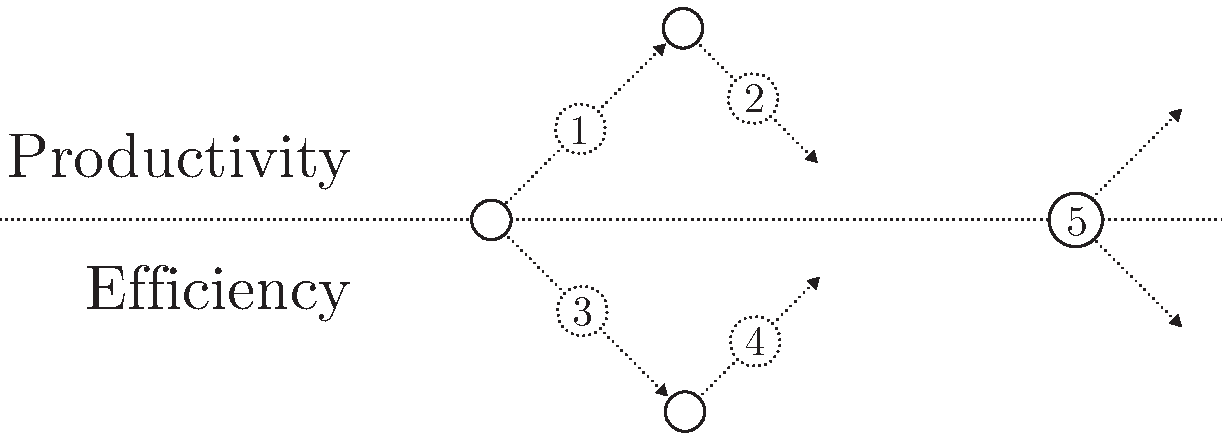
\includegraphics[width=0.6\textwidth]{../ressources/state-of-the-art.pdf}
\end{center}
\end{figure}

\subsection{Web Compliance}

TODO




